\chapter{Report}
\section{a}
The Relationships between Discharge and $\Delta S$ is shown in \autoref{fig:relationship}.
\begin{figure}[htpb]\centering
	\subfigure[]{
		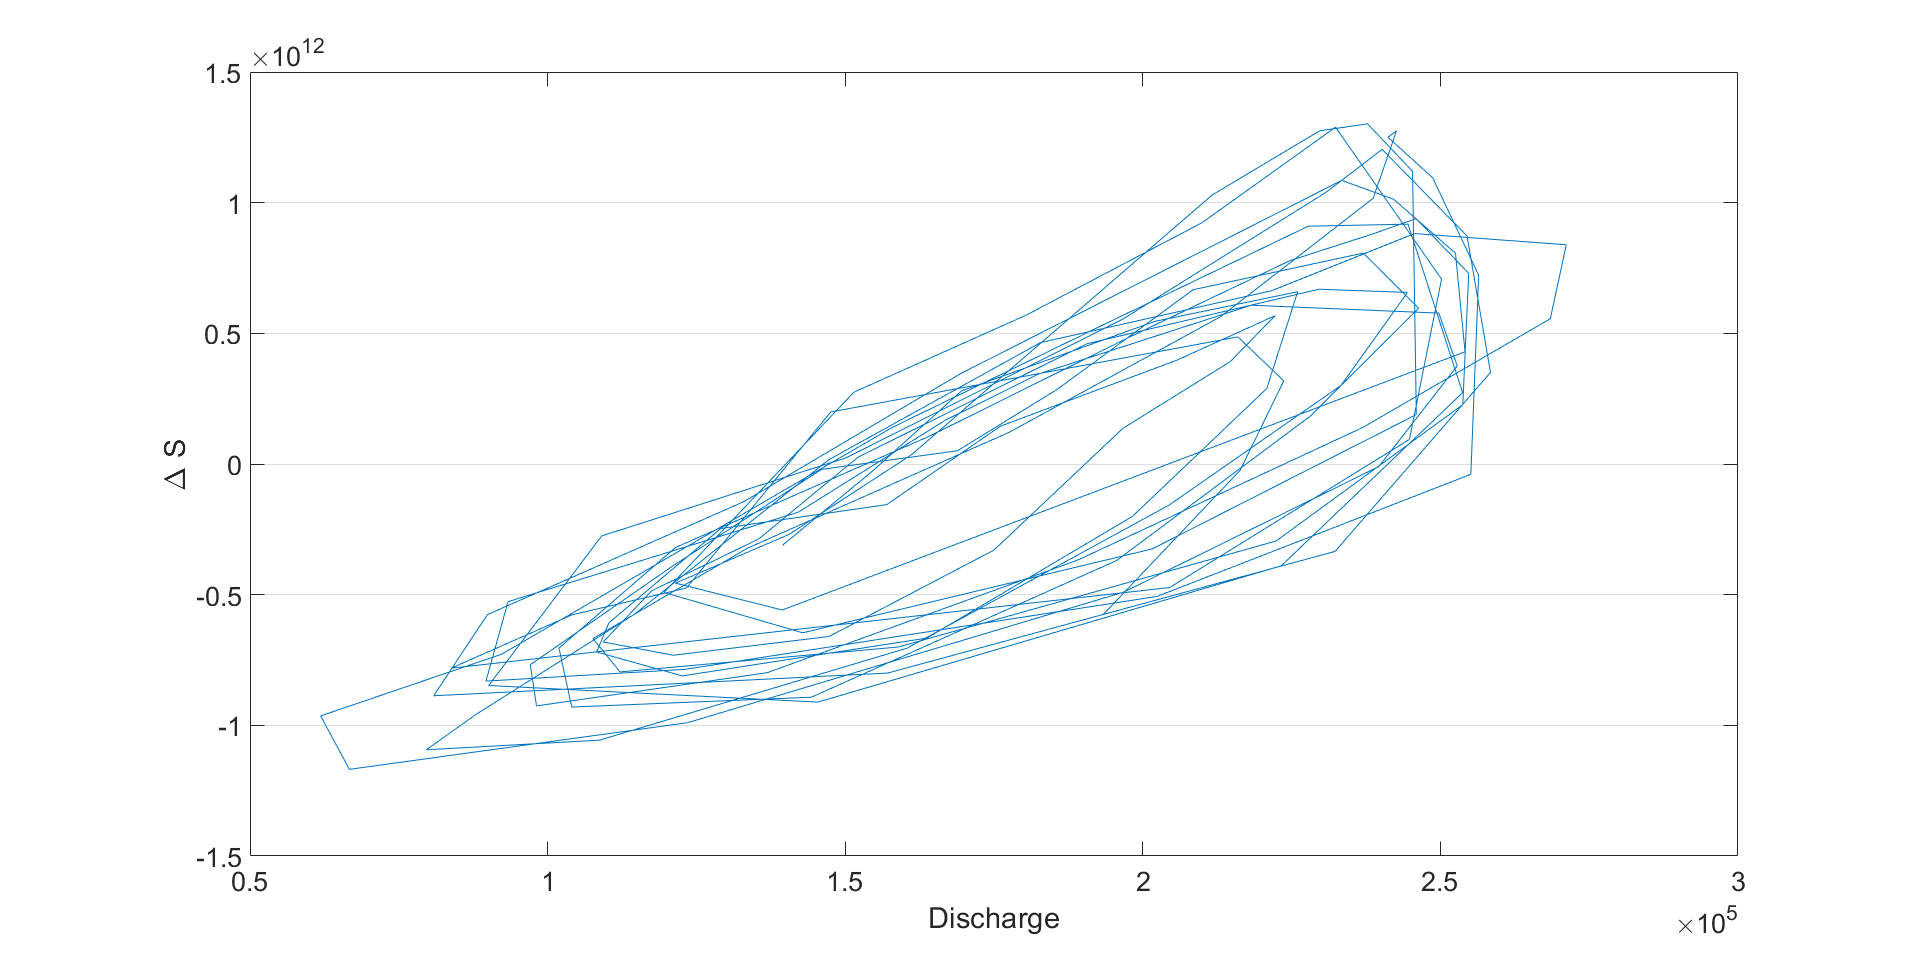
\includegraphics[width=0.9\textwidth]{relationship.png}}
	\caption{}
	\label{fig:relationship}
\end{figure}
\section{b}
\begin{equation*}
	\frac{dR}{dt} + \frac{R}{\tau} = \omega^2_n S
\end{equation*}
\section{c}
\begin{gather*}
	\frac{R_t - R_{t-1}}{\Delta t} + \frac{R_t}{\tau} = \omega^2_n S_t \\
\end{gather*}
If we take $\Delta t$ as 1 unit.
\begin{gather*}
	R_t - R_{t-1} + \frac{R_t}{\tau} = \omega^2_n S_t \\
	\left(1+\frac{1}{\tau}\right) R_{t} = R_{t-1} +  \omega^2_n S_t \\
	R_{t} = \frac{\tau}{\tau + 1} R_{t-1} + \frac{\tau \omega_n^2}{\tau + 1}S_t
\end{gather*}
\section{d}
After solve this ODE:
\begin{gather*}
	R(t_{n+1}) = R(t_{n}) e^{\frac{\Delta t}{\tau}} + \bar{S}(t_{n}) \cdot \omega^2 \tau (e^{\frac{\Delta t}{\tau}} - 1) \\
	R(t_{n+1}) = R(t_{n}) e^{\frac{\Delta t}{\tau}} + \left(S_0 + \Delta S(t_{n})\right) \cdot \omega^2 \tau (e^{\frac{\Delta t}{\tau}} - 1)
\end{gather*}
\section{Part 2}
before from CSR, after JPL
\begin{gather*}
	d \begin{bmatrix}
		\Delta S\\
		R
	\end{bmatrix} = \begin{bmatrix}
	0 & -1 \\
	\omega^2 & -\frac{1}{\tau}
\end{bmatrix} \begin{bmatrix}
\Delta S\\
R
\end{bmatrix} + \begin{bmatrix}
0 & 1 & -1 \\
\omega^2 & 0 & 0
\end{bmatrix} \begin{bmatrix}
S_{0}\\
P\\
ET
\end{bmatrix} \\
\begin{bmatrix}
	\Delta S_{measured} \\
	R_{measured}
\end{bmatrix} = \begin{bmatrix}
1 & 0 \\
0 & 1
\end{bmatrix} \begin{bmatrix}
\Delta S_{predict} \\
R_{predict} 
\end{bmatrix} 
\end{gather*}
which means
\begin{gather*}
	\begin{bmatrix}
		\Delta S_{n+1} \\
		R_{n+1}
	\end{bmatrix} = \begin{bmatrix}
	1 & -1 \\
	\omega^2 \tau (e^{\frac{\Delta t}{\tau}} - 1) & e^{\frac{\Delta t}{\tau}} \end{bmatrix} \begin{bmatrix}
		\Delta S_{n} \\
		R_{n}
	\end{bmatrix} + \begin{bmatrix}
	0 & 1 & -1\\
	\omega^2 \tau (e^{\frac{\Delta t}{\tau}} - 1) & 0 & 0
\end{bmatrix} \begin{bmatrix}
S_0 \\
P \\
ET
\end{bmatrix} \\
\begin{bmatrix}
	\Delta S_{measured} \\
	R_{measured}
\end{bmatrix} = \begin{bmatrix}
	1 & 0 \\
	0 & 1
\end{bmatrix} \begin{bmatrix}
	\Delta S_{predict} \\
	R_{predict} 
\end{bmatrix} 
\end{gather*}
Variance for $R$, I have $R$ from 1968.
\begin{gather*}
	\sigma^2_{R_{January}} = \frac{1}{n-1}\sum (R_{i,January} - \bar{R}_{January})^2
\end{gather*}